\chapter{Clusters and Groups of Galaxies}

Galaxies in the universe do not exist in isolation; instead, they exhibit a remarkable large-scale structure, clustering into distinctive patterns known as groups or clusters. This non-uniform distribution creates a cosmic web of matter, giving rise to both enormous physical features and intriguing observational artifacts. The following figure visualizes this rich tapestry of galaxy locations throughout the cosmos:

\begin{minipage}{0.6\textwidth}
    \centering
    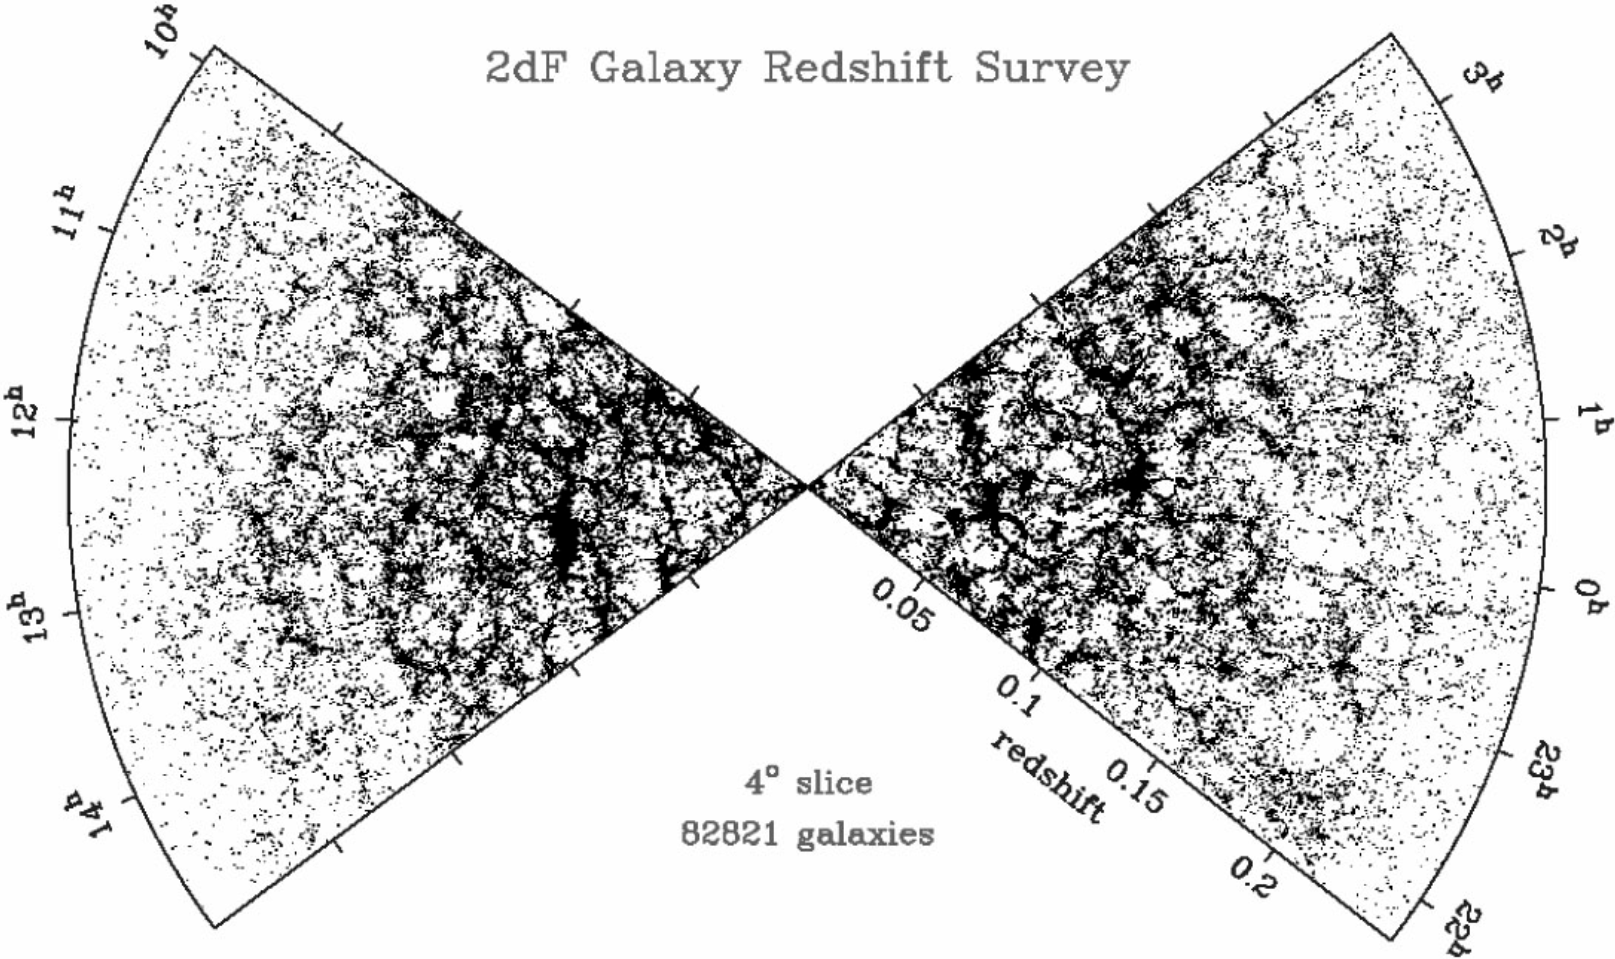
\includegraphics[width=\textwidth]{assets/gal-dist.png}
\end{minipage}%
\hfill
\begin{minipage}{0.37\textwidth}
    \captionof{figure}{Distribution of galaxies in the universe, highlighting large-scale structures. Among these structures, some are genuinely vast aggregations of galaxies (such as the famous \textit{Great Wall}) while others (like the \textit{Finger of God}), are illusions caused by peculiar motions of galaxies within clusters. The latter appear as elongated features in redshift space due to high internal velocities along the observer's line of sight, not because of their true physical extension.}
\end{minipage}%


\begin{tipsblock}[Galaxy distribution]
    In regions of high redshift, galaxies appear less densely packed than at low redshift. This apparent sparsity arises because more distant galaxies have lower apparent brightness and are, therefore, harder to detect with flux-limited surveys, introducing a selection effect.
\end{tipsblock}

\section{Systems of Galaxies: A First Approach}

Aggregations of galaxies are generally categorized based on their richness and scale:

\vspace{0.3em}

\begin{minipage}{0.49\textwidth}
    \textbf{Groups of Galaxies}
    \begin{itemize}
        \item Number of members: $N \lesssim 50$
        \item Diameter: $D \lesssim 1.5\, h^{-1}$
        \item Total mass: $M \lesssim 3 \times 10^{13}\, M_{\odot}$
        \item Intra-group gas temperature: $T_x \sim 1 \text{-} 3\ \mathrm{keV}$
        \item Velocity dispersion: $\sigma_v \sim 200 \text{-} 300\, \mathrm{km/s}$
    \end{itemize}
\end{minipage}%
\hfill
\begin{minipage}{0.49\textwidth}
    \textbf{Clusters of Galaxies}
    \begin{itemize}
        \item Number of members: $N \gtrsim 50$
        \item Diameter: $D \gtrsim 1.5\, h^{-1}$
        \item Total mass: $M \gtrsim 3 \times 10^{14}\, M_{\odot}$
        \item Intra-cluster gas temperature: $T_x \sim 4 \text{-} 10\ \mathrm{keV}$
        \item Velocity dispersion: $\sigma_v \sim 400 \text{-} 1000\, \mathrm{km/s}$
    \end{itemize}
\end{minipage}

\vspace{0.7em}

Clusters of galaxies represent the largest gravitationally bound structures in the known universe. Their typical physical extent is characterized by the \textbf{Abell radius}:

$$
    R_{\mathrm{Abell}} = 1.5\, h_{100}^{-1} \ \mathrm{Mpc}
    \qquad \rightarrow \qquad
    1.5 \cdot \frac{100}{70}\, h_{70}^{-1} \ \mathrm{Mpc}
$$

Clusters and groups are multi-component systems comprising several key constituents:
\begin{itemize}
    \item \textbf{Hot gas} ($\sim$15–20\%): The intracluster medium (ICM) is filled with hot, ionized gas at temperatures around $T \sim 3 \times 10^7$ K. This plasma emits strong X-rays and often contains more baryonic matter than all the stars in the cluster's galaxies combined.
    \item \textbf{Dark matter} ($\sim$80\%): Dark matter dominates the mass budget, as inferred from observations of galaxy motions, X-ray gas dynamics, and gravitational lensing effects.
    \item \textbf{Stars} ($\sim$3-5\%): The stellar component within galaxies are only a small fraction of the total mass.
\end{itemize}

\subsection{Secondary Distance Measuring (Extragalactic distance ladder)}

To determine the distances to remote galaxies and galaxy clusters, astronomers must rely on secondary distance indicators. These methods are calibrated using primary indicators (such as Cepheid variables) in nearby galaxies and can then be extended to much deeper cosmic scales where individual stars can no longer be clearly resolved.

\vspace{-0.5em}

\begin{figure}[H]
    \centering
    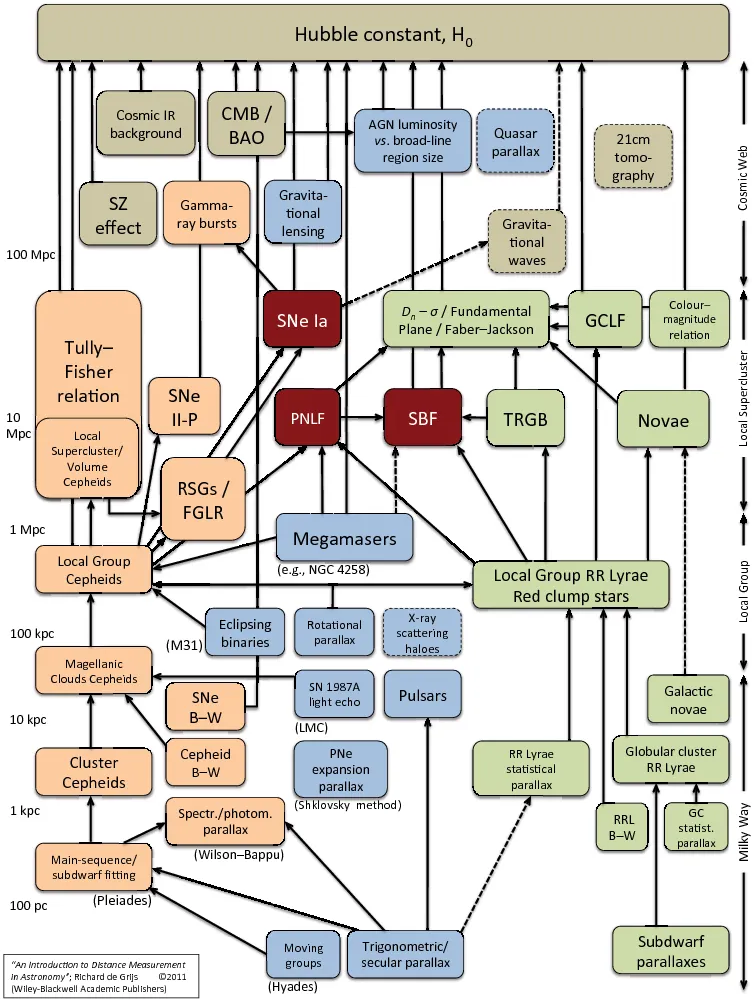
\includegraphics[width=0.77\textwidth]{assets/distance-ladder.png}

    \vspace{-0.3em}

    \caption{\centering The extragalactic distance ladder}
\end{figure}

\subsubsection{Surface Brightness Fluctuation (SBF)}

The SBF technique exploits the fact that, for nearby galaxies ($z \sim 0$), the surface brightness appears roughly constant, but statistical variations in the number of resolved stars per resolution element become detectable. The underlying idea:

\begin{itemize}
    \item For a nearby galaxy, each pixel (resolution element) covers only a small number of stars, so pixel-to-pixel fluctuations are significant.
    \item For a distant galaxy, each pixel contains light from many stars, so the total surface brightness is smoother and fluctuations are smaller.
\end{itemize}

The statistical (Poisson) error associated with counting $N$ stars in a pixel is $\sqrt{N}$, giving a relative fluctuation of $1/\sqrt{N}$. Therefore, as the number of stars per pixel increases with distance, the surface brightness becomes smoother and the observed fluctuations diminish.

Despite its conceptual simplicity, the SBF technique is a powerful and widely adopted approach in observational cosmology, and is currently used in major projects such as the Euclid mission.

\subsubsection{BW (Baade-Wesselink) Method}

The Baade-Wesselink method is applied to objects whose radii change with time (objects that expand or pulsate, such as Cepheids or supernovae).

Recall the relation for luminosity:
$$
L = 4\pi R^2 \sigma T_{\mathrm{eff}}^4
$$
By tracking temporal changes, we can determine both the radius of the object and how it evolves. Specifically, the difference in radius between two epochs, $T_0$ and $T_1$, is given by:
$$
\Delta R = R_1 - R_0 = p \int_{T_0}^{T_1} v_{los}(t)\, dt
$$
where $p$ is a parameter that takes into account the shape of the object (e.g. if a sphere, then $p = 1$).

The change in absolute and apparent magnitude can be expressed as:
$$
m_1 - m_0 = M_1 - M_0 = -5 \big[\log(R_0 + \Delta R) - \log R_0\big] = -10 [\log T_1 - \log T_0]
$$

So, the initial radius can be determined as a function of measured or derived quantities:
$$f
R_0 = f(m_0, m_1, \Delta R, T_0, T_1)
$$

\begin{minipage}{0.6\textwidth}
    This method is widely employed to estimate distances to supernovae, particularly those of Type Ia. By analyzing their light curves, one can determine the timescale around maximum luminosity ($\Delta t \sim L_{max}$). The value of $L_{max}$ provides the absolute magnitude of the supernova; when this is compared to the observed apparent magnitude, the distance modulus, and thus the distance, can be derived.
\end{minipage}
\hfill
\begin{minipage}{0.35\textwidth}
    \centering
    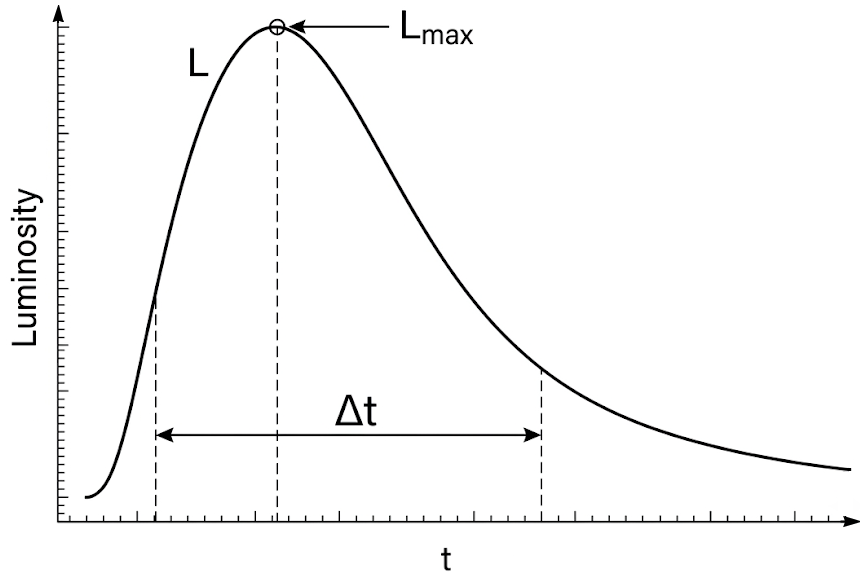
\includegraphics[width=\textwidth]{assets/supernovae.png}
\end{minipage}

While this method can be useful, it is important to note that it \textit{does not take extinction into account}.

\subsubsection{Hubble's Law}

One of the most profound discoveries in modern astronomy was made by Edwin Hubble in 1928: he observed that distant galaxies, on average, appear to be moving away from us, and that their recessional velocity is proportional to their distance. This relationship, now called \textbf{Hubble's Law}, revealed that the Universe itself is expanding.
Mathematically, the law is expressed as:
$$
v = H_0\, d
$$

where $v$ is the galaxy's recessional velocity (at low redshift $v\sim cz$), $d$ is its distance from the obs and $H_0$ is the \textbf{Hubble constant}, setting the rate of expansion of the Universe.

\begin{minipage}{0.57\textwidth}
    When we plot Hubble's law by displaying the observed velocities of galaxies versus their distances, we often notice elongated vertical structures: these are known as the \textbf{Fingers of God}, introduced earlier. 
    \smallskip

    These features do not represent actual physical elongations in space; rather, they are artifacts produced by the high internal (peculiar) velocities of galaxies within galaxy clusters.
\end{minipage}%
\hfill
\begin{minipage}{0.4\textwidth}
    \centering
    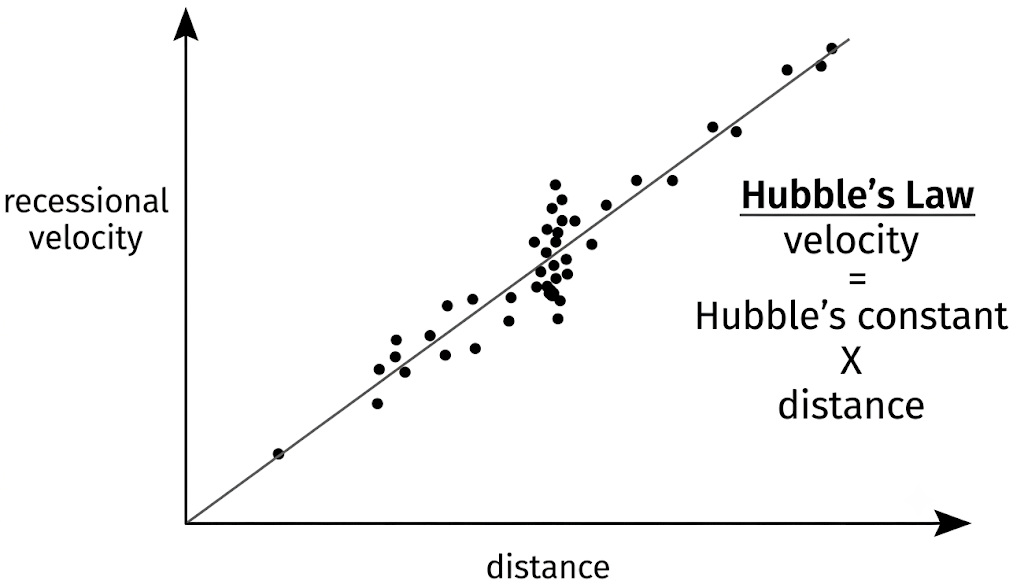
\includegraphics[width=\textwidth]{assets/hubble-law.png}
    \captionof{figure}{\centering of Hubble's Law.}
\end{minipage}

\smallskip

The Hubble constant quantifies how fast the Universe is expanding at the current epoch. Its units are typically given in $\mathrm{km\, s^{-1}\, Mpc^{-1}}$, i.e., kilometers per second of recession for every megaparsec of distance.

Historically, measurements of $H_0$ have varied significantly depending on the observational technique and wavelength used. For example, around 1990:
\begin{itemize}
    \item \textbf{Optical observations:} $H_0 = 100\, \mathrm{km\,s^{-1}\,Mpc^{-1}}$
    \item \textbf{X-ray observations:} $H_0 = 50\, \mathrm{km\,s^{-1}\,Mpc^{-1}}$
\end{itemize}
More recent measurements, such as those derived from observations of the Cosmic Microwave Background (CMB, often using missions like Planck), yield:
\begin{itemize}
    \item \textbf{CMB (modern cosmology):} $H_0 \sim 70\, \mathrm{km\,s^{-1}\,Mpc^{-1}}$
\end{itemize}

To standardize results and facilitate comparisons, it is common to write:
$$
H_0 = h \times 100\, \mathrm{km\,s^{-1}\,Mpc^{-1}}
$$
where $h$ is a dimensionless scaling factor (typically $h \sim 0.7$).

\begin{observationblock}[The Hubble Tension]
    Modern measurements of the Hubble constant $H_0$ using different techniques yield discrepant values. This ongoing discrepancy is known as the \textbf{Hubble (Cosmological) Tension}, and it represents one of the most intriguing unsolved problems in cosmology.
\end{observationblock}

A further key concept in the study of galaxy clusters is the \textbf{dimensionless Hubble parameter as a function of redshift}:

$$
E(z) \equiv \frac{H(z)}{H_0}
$$

where $H(z)$ is the Hubble parameter at a given redshift $z$, and $H_0$ is the Hubble constant today. $E(z)$ parametrizes the expansion rate of the Universe at different cosmic epochs and frequently appears in cosmological calculations.

\medskip

Another fundamental quantity is the \textbf{critical density} required for the Universe to be spatially flat (i.e., marginally bound). This is defined as:

$$
\rho_c \equiv \frac{3 H_0^2}{8 \pi G}
$$

where $G$ is the gravitational constant. If the mean matter density of the Universe $\rho$ is greater than $\rho_c$, the Universe is closed and will eventually recollapse; if $\rho < \rho_c$, it will expand forever. Modern measurements suggest $\rho \approx \rho_c$ within a few percent, implying a nearly flat Universe.

On smaller (galaxy and cluster) scales, gravitational collapse can occur wherever the mean density exceeds the local critical value. In the context of structure formation, regions where the average density exceeds a threshold (often set to $200$ times the critical density) are expected to have stopped expanding with the Universe and undergone gravitational collapse:

$$
\langle \rho \rangle = 200\, \rho_c \quad \Rightarrow \quad \text{Gravitational Collapse}
$$

This threshold value is used to define the characteristic radius of a galaxy cluster, denoted as $R_{200}$: the radius within which the mean density is $200$ times the critical density.

Statistical surveys indicate that $\gtrsim 50\%$ of all galaxies reside in \textbf{groups} and $\sim 5\%$ of galaxies are located in rich \textbf{clusters}.

\section{Groups of Galaxies}

\subsection{The Local Group}

The \textbf{Local Group} is a gravitationally bound collection of galaxies, extending over approximately $1-2$~Mpc, and represents our immediate ocosmic neighborhood. It contains about 35--50 known members with luminosities $L \lesssim L^*$, and a total mass estimated at $M \sim 3 \times 10^{12}~M_{\odot}$. The Local Group is dominated by three prominent spiral galaxies:

\begin{center}
\small
\renewcommand{\arraystretch}{1.3}
\begin{tabular}{lccc}
 & \textbf{MW (Milky Way)} & \textbf{M31 (Andromeda)} & \textbf{M33 (Triangulum)} \\
\hline
Hubble type & $SB_{bc}$ & $S_b$ & $S_c$ \\
$M_B$ & $-20$ & $-21.2$ & $-18.9$
\end{tabular}
\end{center}

\textbf{M31} (\textbf{Andromeda}) is the most massive and luminous galaxy in the group, situated at a distance of $D = 770$~kpc from the Milky Way and approaching us at $v \sim 120$~km/s (i.e., blueshifted). This relative motion predicts a possible collision and merger with our Galaxy in about $6 \times 10^9$ years.

\smallskip

In addition to the primary spirals, the Local Group contains numerous dwarf galaxies, many of which are associated with the Magellanic Stream, a prominent, elongated trail of neutral hydrogen gas that was drawn out from the Magellanic Clouds through tidal interactions with the Milky Way. Intriguingly, the majority of these dwarf companions are distributed along a thin plane, which is oriented nearly perpendicular to the disk of the Galaxy.

\begin{figure}[H]
    \centering
    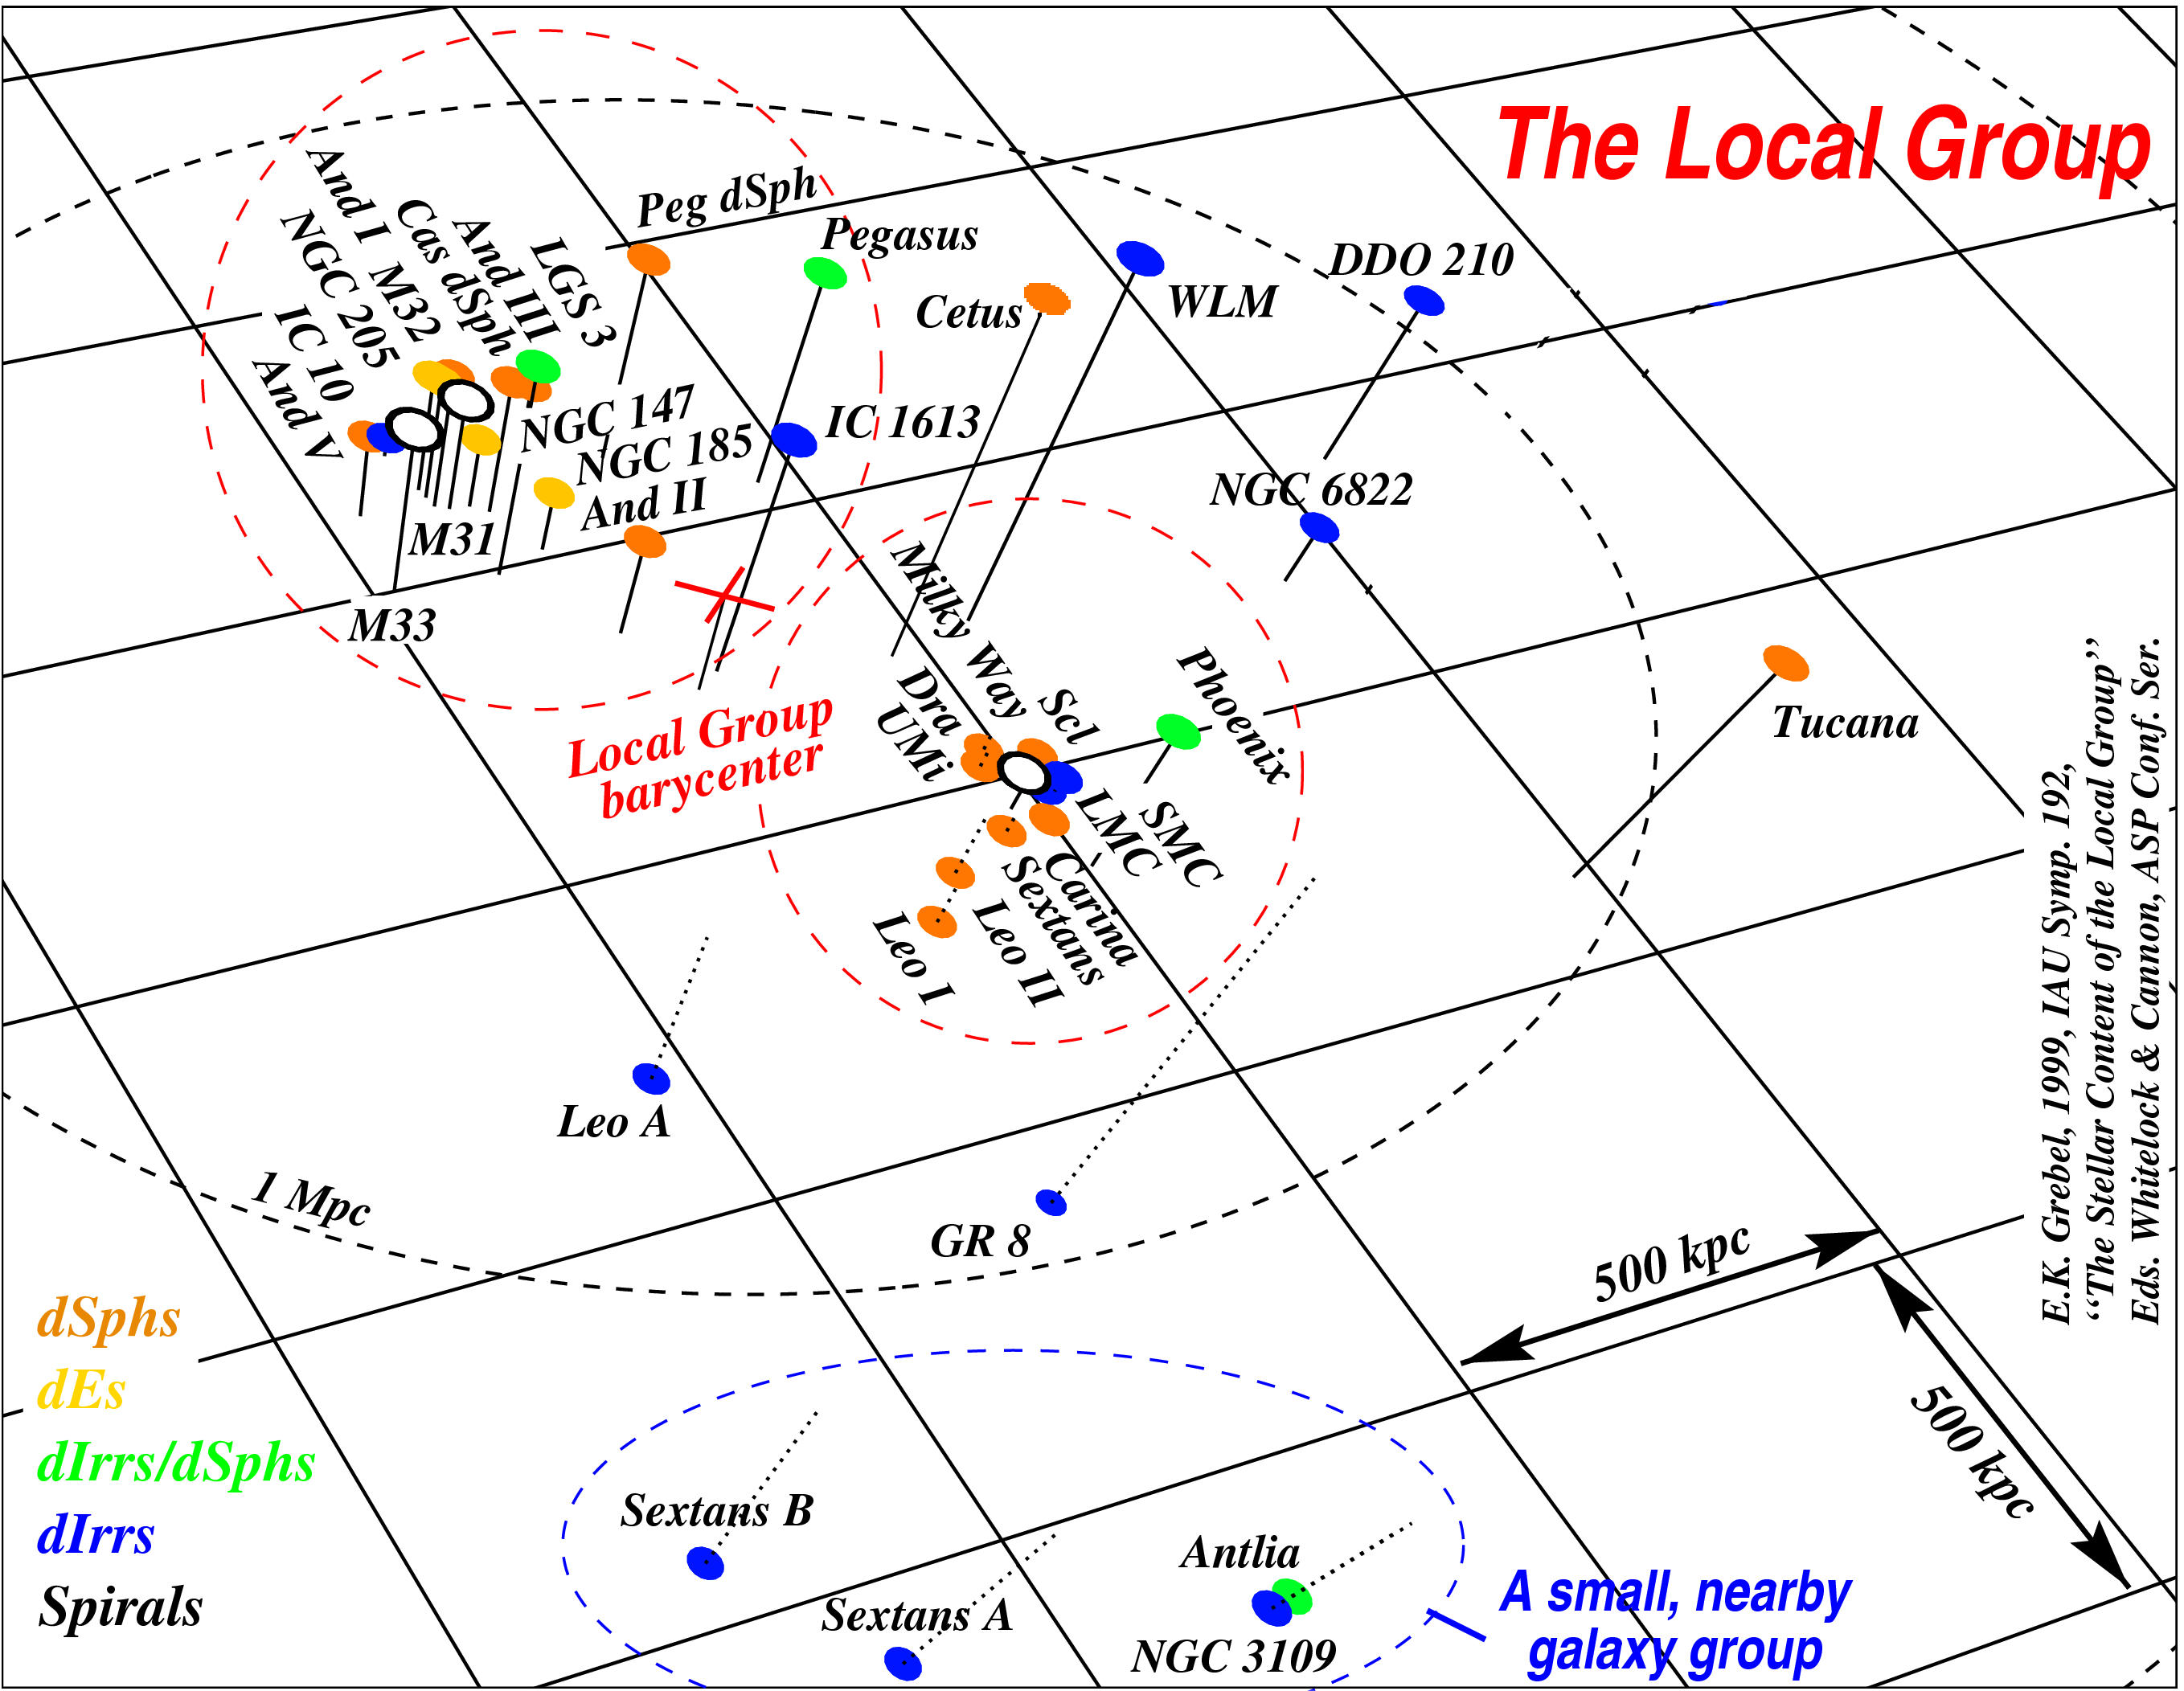
\includegraphics[width=0.6\textwidth]{assets/local-group.jpg}
    \caption{\centering Schematic representation of the Local Group, showing major and satellite galaxies \cite{grebel}.}
\end{figure}

\subsubsection{Mass Estimation of the Local Group}

The total luminosity and mass of the Local Group are overwhelmingly dominated by the Milky Way and Andromeda, which together account for approximately 90\% of the group emission and mass:
$$
M_{\mathrm{LG}} = M_{\mathrm{MW}} + M_{\mathrm{M31}} \sim 0.9\,L_{\mathrm{LG}} \sim 0.9\,M_{\mathrm{LG}}
$$

A classical approach to estimate the total dynamic mass of the Local Group is the \bfit{two body timing argument}. This argument posits that in the early phases of the Universe, the Milky Way and Andromeda were close together and initially took part in the general Hubble expansion. Over time, their mutual gravitational attraction decelerated their relative separating motion until it came to a complete halt. This turnaround point occurred at a time $t_{max}$, at which the two galaxies reached their maximum separation $r_{max}$. From that moment they have been falling back towards each other.

Starting from the conservation of specific energy for a radial orbit:
$$
\frac{1}{2} v^2 - \frac{G M}{r} = C
$$
At the point of maximum separation ($t_{max}$, $r_{max}$), the relative velocity is zero ($v = 0$), which allows us to determine the constant of integration $C$:
$$
C = - \frac{G M}{r_{max}}
$$
Substituting this back into the energy equation and isolating the velocity term $v = dr/dt$, we obtain:
$$
\dfrac 12 \left( \dfrac{dr}{dt} \right)^2 = \dfrac {G M}{r} - \dfrac{G M}{r_max}
$$
We can rearrange this differential equation to solve for the time interval $dt$:
$$
(dt)^2 = \frac{(dr)^2}{2 GM} \left( \frac{1}{\frac{1}{r} - \frac{1}{r_{max}}} \right) \qquad \Rightarrow \qquad dt = \frac{dr}{\sqrt{2 GM}} \frac{1}{\sqrt{\frac{1}{r} - \frac{1}{r_{max}}}}
$$
Integrating from the initial state at $t=0$ to the turnaround time $t_{max}$ gives the total expansion time:
$$
t_{max} = \int_0^{t_{max}} dt = \int_0^{r_{max}} \dfrac{dr}{\sqrt{2 GM} \sqrt{\dfrac{1}{r} - \dfrac{1}{r_max}}} = \dfrac {\pi}{2} \dfrac{r_{max}^{3/2}}{\sqrt{2 GM}}
$$

where the result is obtained using the Wolfram rule:
$$
\int_0^a \dfrac 1{\sqrt{\frac 1x - \frac 1a}} dx = \dfrac {\pi}{2} a^{3/2}
$$

By inverting this relation, we can express the maximum separation radius as a function of the turnaround time and the total mass:
$$
r_{max} = \left( \dfrac{2 \sqrt{2 G M}}{\pi} t_{max} \right)^{2/3}
$$
Substituting this $r_{max}$ back into the original energy conservation equation yields the velocity as a function of the current separation $r$ and the turnaround time $t_{max}$:
$$
\dfrac {v^2}2 = \dfrac {G M}{r} - \dfrac 12 \left( \dfrac{ \pi GM}{t_{max}} \right)^{2/3} \qquad \Rightarrow \qquad v = f(M, t_{max})
$$

We can roughly estimate the timescales. The total time since the Big Bang is $t_0$, and the total time until the future collision is $t_{collapse}$, such that the full orbit takes $2 t_{max} = t_0 + t_{collapse}$. Using the presently observed values for the separation distance 770 Mpc and the relative approach velocity 120 km/s, we find:

$$
\frac{r(t_o)}{v(t_0)} = \frac{D_{obs}}{v_{obs}} = \frac{770 kpc}{120 km/s} = 6 \cdot 10^9 yr
\qquad \Rightarrow \qquad t_{max} \sim \frac 12 t_0 + \frac 12 \frac{D_{obs}}{v_{obs}} \sim 10^{10} yr
$$

This kinematic ratio implies a turnaround time $t_{max}$ on the order of $10^{10}$ years. By inserting these observed values back into our velocity function, we finally isolate the total dynamical mass of the Local Group:
$$
M = f(\nu, t_{max}) = 3 \cdot 10^{12} M_{\odot}
$$

Comparing this immense dynamical mass to the observed luminosity yields a mass to light ratio of approximately 70 $M_{\odot}/L_{\odot}$. Because the visible stars and gas in the Milky Way and Andromeda account for only about 5\% of this estimated mass, the two body timing argument provides strong, independent kinematic evidence for the existence of massive dark matter halos surrounding both galaxies.

\subsection{Sculptor and M81 Groups}

Beyond the Local Group, the Universe is populated by numerous other small galaxy aggregates. The most immediate neighboring system is the \textbf{Sculptor Group}, a loose collection of about six primary members located at a distance of approximately 1.8 Mpc. 

Slightly further out lies the \textbf{M81 Group}, situated at a distance of about 3.1 Mpc. This group contains roughly eight prominent galaxies, interacting dynamically in a manner similar to our own Local Group.

\section{Clusters of Galaxies}

While groups contain dozens of galaxies, \textbf{clusters of galaxies} are the largest gravitationally bound structures in the Universe, often containing hundreds or thousands of members. They provide crucial laboratories for studying both galaxy evolution in dense environments and the cosmological distribution of dark matter.

\bigskip

Two well known local examples illustrate the diversity of these structures:

\medskip

\begin{center}
\begin{minipage}{0.5\textwidth}
    \begin{itemize}
        \item The \textbf{Virgo Cluster}, classified as an \bfit{irregular cluster}, is the closest major cluster, located at a distance of roughly 16 Mpc. It spans an immense 10 degrees of sky and contains roughly 250 large galaxies and 2000 smaller ones, heavily dominated by the giant elliptical galaxy M87 at its center.
        \item The \textbf{Coma Cluster}, in contrast, is a prototypical example of a \bfit{regular cluster}. It is much larger and denser, located at a distance of 90 Mpc with a redshift of approximately $z = 0.023$. Coma is a very rich, highly concentrated cluster containing thousands of galaxies.
    \end{itemize}
\end{minipage}\hfill
\begin{minipage}{0.47\textwidth}
        \centering
        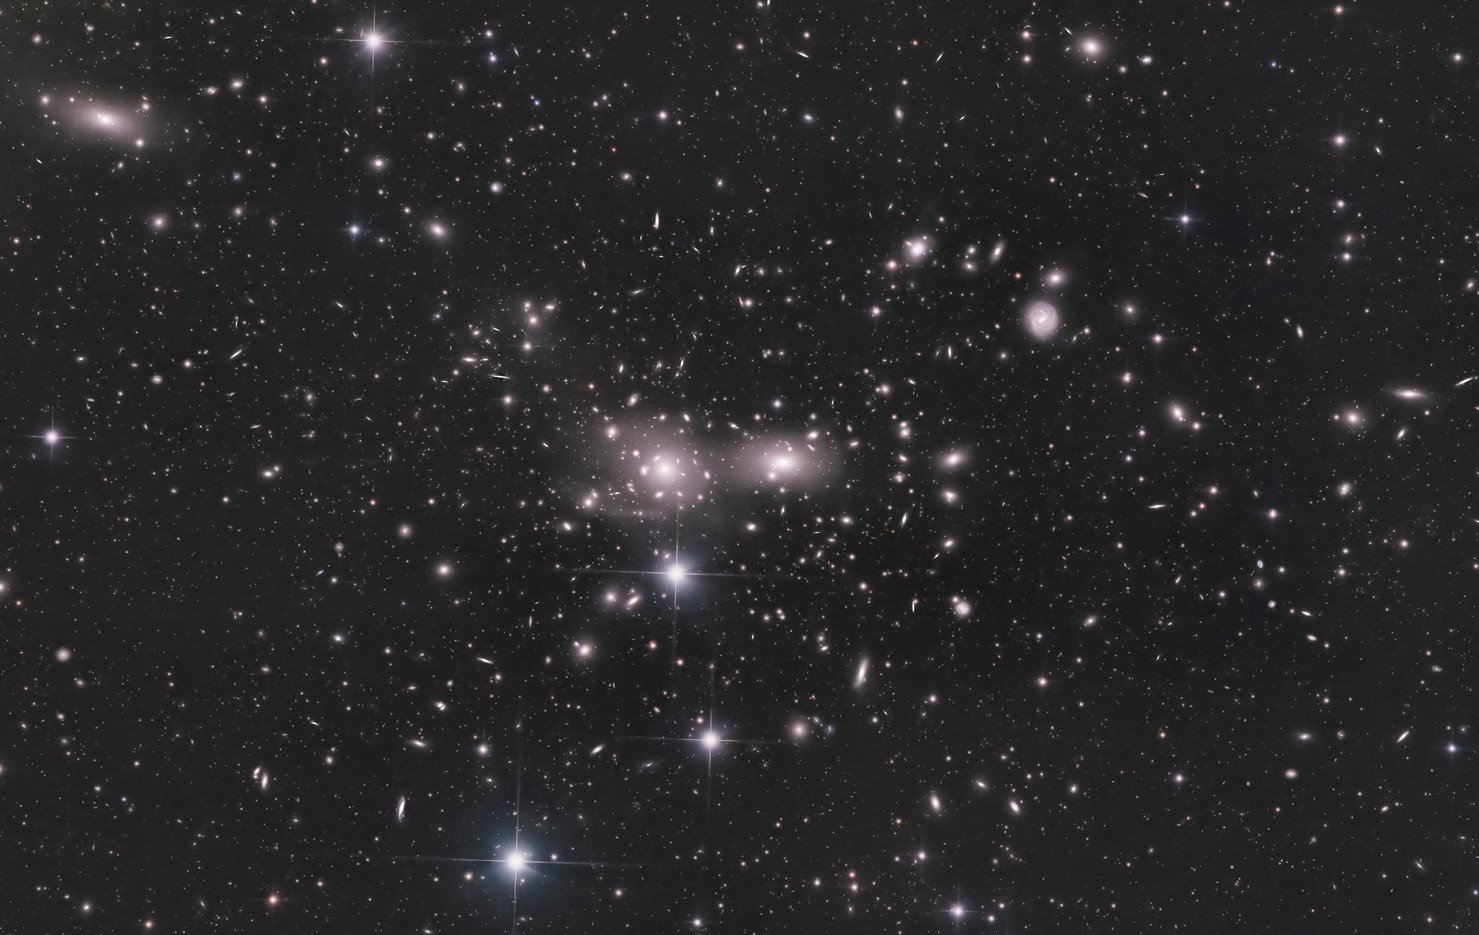
\includegraphics[width=\textwidth]{assets/coma.png}
        \captionof{figure}{Optical image of the Coma Cluster, showing hundreds of galaxies strongly concentrated toward the core \cite{coma_2024}.}
\end{minipage}
\end{center}

\section{Catalogues of Groups and Clusters}

\subsection{Abell Catalogue}

The Abell catalogue is an optical catalogue, identifying regions of the sky that show an overdensity of galaxies. These regions were identified visually by examining photographic plates from the Palomar Observatory Sky Survey (POSS). The Galactic disk region was omitted because observing galaxies there is particularly challenging, due to extinction and high stellar density.

\subsubsection{Abell Criteria}

The criteria for an Abell cluster include:
\begin{enumerate}
    \item The cluster must contain more than 50 galaxies.
    \item Galaxies are counted within the magnitude interval $m_3 \leq m \leq m_3+2$, where $m_3$ is the magnitude of the third brightest member.
    \item The galaxies must be located within a circular area of angular radius:
    $$
    \theta_A = \frac{1.'7}{z}
    $$
    where $z$ is the estimated redshift.

    \item The corresponding physical radius (based on the assumption that the luminosity of the tenth brightest galaxy is similar across all clusters) is:
    $$
    R_{Abel} = 1.5 h^{-1}~\mathrm{Mpc}
    $$

    \item The redshift range for selecting Abell clusters is $0.02 \leq z \leq 0.2$: the lower limit ensures the cluster fits on a single POSS photoplate, the upper limit reflects the sensitivity of the plates.
\end{enumerate}

\subsubsection{Problems in the Optical Search for Clusters}

Selecting galaxy clusters based on overdensities in projected sky positions introduces several complications, especially when using these catalogues for statistical analysis.

Some important definitions include:
\begin{itemize}
    \item \textbf{Completeness}: All objects satisfying the selection criteria should be included in the catalogue. In practice, it may only reach $\dfrac{N_{obs}}{N_{true}} \le 1$.
    \item \textbf{Purity}: The fraction $\dfrac{N_{obs} - N_{false}}{N_{obs}} \le 1$ should be maximized, meaning the catalogue should contain as few false detections as possible.
    Since a galaxy cluster is inherently a three-dimensional structure, while optical searches rely on two-dimensional projections, \bfit{projection effects} are unavoidable: random alignments along the line of sight can mimic genuine clusters.

    \item \textbf{Richness}: Defined as the number of galaxies within the cluster.
\end{itemize}

Additionally, fluctuations in foreground galaxy density can cause genuine high-redshift clusters to be overlooked, or insignificant fluctuations to be misidentified as clusters.

For these reasons, the Abell catalogue is neither fully complete nor fully reliable.

\subsubsection{Abel Classes}

There are two types of classification in the Abell catalogue: six richness classes (numbered 0 to 5) according to the number of cluster member galaxies, and six distance classes based on the apparent magnitude of the tenth brightest galaxy, reflecting the cluster's estimated redshift.

\begin{table}[H]
    \centering
    \setlength{\tabcolsep}{18pt}
    \begin{minipage}[t]{0.49\textwidth}
        \centering
        \footnotesize
        \captionsetup{justification=centering}
        \caption{Abell's richness classes}
        \label{tab:abell-richness}
        \renewcommand{\arraystretch}{1.15}
        \begin{tabular}{>{\bfseries}c c c}
        $R$ & $N$ & Clusters \\
        \hline
        0 & 30--49     & $\geq 1000$ \\
        1 & 50--79     & 1224 \\
        2 & 80--129    & 383 \\
        3 & 130--199   & 68 \\
        4 & 200--299   & 6 \\
        5 & $\geq 300$ & 1 \\
        \end{tabular}
    \end{minipage}%
    \hfill
    \setlength{\tabcolsep}{10pt}
    \begin{minipage}[t]{0.49\textwidth}
        \centering
        \footnotesize
        \captionsetup{justification=centering}
        \caption{Abell's distance classes}
        \label{tab:abell-distance}
        \renewcommand{\arraystretch}{1.15}
        \begin{tabular}{>{\bfseries}c c c c}
        $D$ & $m_{10}$ & $\langle z \rangle$ & $N(R\!\geq\!1)$\\
        \hline
        1 & 13.3--14.0 & 0.0283 & 370 \\
        2 & 14.1--14.8 & 0.0400 & 444 \\
        3 & 14.9--15.5 & 0.0595 & 427 \\
        4 & 15.6--16.2 & 0.0776 & 346 \\
        5 & 16.3--16.9 & 0.0997 & 366 \\
        6 & 17.0--18.0 & 0.1198 & 921 \\
        \end{tabular}
    \end{minipage}
\end{table}

\subsection{Morphological Classification of Clusters}

\subsubsection{Rood-Sastry Classification}

The morphological classification by Rood and Sastry divides galaxy clusters into several categories:

\begin{minipage}{0.65\textwidth}
    \begin{itemize}[itemsep=0.5em]
        \item \textbf{cD}: Dominated by a large, central \textit{cD galaxy} surrounded by smaller galaxies at the cluster's core.
        \item \textbf{B}: Marked by a \bfit{binary} system, two bright dominant galaxies situated at the center.
        \item \textbf{L}: The brightest galaxies are arranged in a nearly \bfit{linear} sequence, forming a prominent chain.
        \item \textbf{C}: Characterized by a concentrated, compact \bfit{single core} of galaxies with considerable central density.
        \item \textbf{F}: Shows a \bfit{flat} or uniform spatial distribution, with galaxies spread across the cluster and weak central concentration.
        \item \textbf{I}: Displays an \bfit{irregular} pattern, lacking a clear structure or dominant core; galaxies are unevenly scattered.
    \end{itemize}
\end{minipage}%
\hfill
\begin{minipage}{0.3\textwidth}
    \centering
    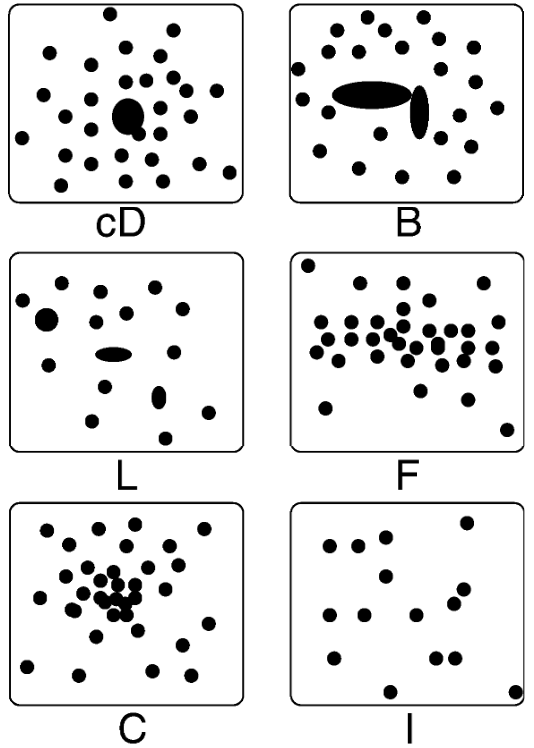
\includegraphics[width=\textwidth]{assets/morph-class.png}

    \vspace{-0.5em}
    \captionof{figure}{Rood-Sastry morphological classification \cite{schneider}}
\end{minipage}

\medskip
% \vspace{-1em}

cD and Binary types are exceptionally luminous in X-rays and contain a high fraction of elliptical galaxies. Linear, flat, core, and irregular types often display various substructures.

\subsubsection{Zwicky-Abell Classification}

\begin{itemize}
    \item \textbf{Regular Clusters}: These clusters are overwhelmingly populated by early-type galaxies, and are typically dominated by a massive central cD galaxy. Their central galaxy density is extremely high, and they often exhibit substantial richness. Structurally, regular clusters are generally well-relaxed and show little to no substructure, indicating a mature dynamical state.
    \item \textbf{Irregular Clusters}: In contrast, irregular clusters contain a significant fraction of spiral galaxies, comparable to the proportion found in the general field galaxy population. Their central regions are much less dense, and they frequently display substructures or evidence of ongoing mergers. These clusters tend to have fewer member galaxies overall and are often dynamically young, still undergoing the process of formation and evolution.
\end{itemize}
